\documentclass[a4paper]{article}
\usepackage[utf8x]{inputenc}
\usepackage[T1]{fontenc}
\usepackage[MeX]{polski}
\usepackage{amssymb}
\usepackage{graphicx}
\usepackage{fancyhdr}
\usepackage{lastpage}

\pagestyle{fancy}
\fancyhf{}
\cfoot{ \thepage \hspace{1pt} / \pageref{LastPage}}
\lhead{Specyfikacja implementacyjna}
\rhead{\texttt{GameOfLife}}

\begin{document}

\begin{titlepage}
	\begin{center}
		\vspace*{5cm}

	        \Huge
        	\textbf{Specyfikacja implemetnacyjna automatu kom\'orkowego}

        	\vspace{1cm}
	        \Huge
        	\texttt{GameOfLife}: Gra w \.zycie Johna Conwaya

    		\vspace{1.5cm}

	        \large
		Aleksandra Michalska, Natalia Olszweska

        	\vfill

	        \vspace{3cm}


		\large 09.03.2021
	\end{center}
\end{titlepage}


\tableofcontents
\newpage

\section{Informacje og\'olne}

\subsection{Opis dokumentu}

\quad Dany dokument koresponduje z poprzedni\k{a} specyfikacj\k{a} - Secyfikacj\k{a} funkcjonaln\k{a}

\subsection{\'Srodowisko implementacyje}
\quad Docelowa gra zosta\l{}a napisana w \'srodowiskach Linuxowych, w j\k{e}zyku C. 


\subsection{Informacje o wy\'swietlanych generacjach}

\quad Wy\'swietlana posta\'c generacji zosta\l{}a utowrzona z dwukolorowych kwadra\'ow. 
Stan \.zywy kom\'orki zosta\l{} oznaczony bia\l{}ym kolorem, natomiast stan martwy kolorem czarnym. 
Kolorowe kwadraty zosta\l{}y wy\'swietlone przy pomocy Unicodu, \.zywa - u2b1c, martwa - u2b1b. 

\section{Opis modu\l{}\'ow}

\subsection{Main}

\quad W module g\l{}\'ownym, dalej \textit{Main}, zosta\l{}a zaimplementowana podstawowa cz\k{e}\'s\'c programu. 
Mo\.za tam odczyta\'c posta\'c struktury pojedy\'nczej \textit{generacji}. 
\textit{Main} odpowiada za obs\l{}ug\k{e} parametr\'ow, czytanie pliku wej\'sciowego oraz zapis ko\'ncowej genracji, a tak\.ze uruchomienie odpowiedniego trybu programu (SBS, FAST). 
Modu\l{} g\l{}\'owny nawi\k{a}zuje do modu\l{}u \textit{Modes}.  

\subsubsection{Struktura generacji}

\quad Struktura \textit{generacji} zawiera: 
\begin{itemize}

	\item zmienn\k{a} \textbf{gen} typu \textbf{int**} - dwuwymiarow\k{a} tablic\k{e} zawieraj\k{a}c\k{a} liczby z zakresu 0-1, oznaczaj\k{a}ce stan danej kom\'orki.
	\item zmienn\k{a} \textbf{r} typu \textbf{int} - oznaczaj\k{a}c\k{a} liczb\k{e} wierszy tablicy.
	\item zmienn\k{a} \textbf{c} typu \textbf{int} - oznaczaj\k{a}c\k{a} liczb\k{e} kolumn tablicy.
	\item zmienn\k{a} \textbf{Nr} typu \textbf{int} - oznaczaj\k{a}c\k{a} liczb\k{e} kolejnej generacji.

\end{itemize}

\subsubsection{Obs\l{}uga parametr\'ow wej\'sciowych}

\quad W module \textit{Main} funkcja \textit{main} pobiera parametry z wywo\l{}ania wsadowego. 
Parametry te nast\k{e}pnie s\k{a} porz\k{a}dkowane i sprawdzne dzi\k{e}ki funkcji \textit{Switch}. 
Dzi\k{e}ki tej funkcji parametry wywo\l{}ania zostaj\k{a} zapisane do zmiennych programu, kt\'ore nast\k{e}pnie przekazywane s\k{a} do poszczeg\'olnych funkcji. 
W przypadku b\l{}\k{e}dnego typu lub zapisu danych zwaracane zostaj\k{a} kody b\l{}\k{e}d\'ow.
Dla u\l{}atwienia dzia\l{}ania programu dla niekt\'orych parametr\'ow zosta\l{}y utowrzone w\l{}asne typy (przy pomocy \textit{enum}), np. dla parametru "-m" typ danych \textit{modes} mo\.ze zawiera\'c warto\'sci \textit{sbs} lub \textit{fast}.

\subsubsection{Odczyt i zapis plik\'ow}

\quad Na podstawie pliku wej\'sciowego utowrzona zostaje pocz\k{a}tkowa genracja, kt\'ora nast\k{e}pnie zostaje przekazana pozosta\l{}ym funkcj\k{a} jako argument.
Ostatnia generacja natomiast zostaje przekazana z powrotem do funkcji \textit{main} przez, wybran\k{a} funkcje trybu jako warto\'s\'c zwracana.
Zostaje ona nast\k{e}pnie zapisana do pliku tekstowego, kt\'orego nazw\k{e} podano przy uruchomieniu programu.

\subsubsection{Uruchomienie odpowiedniego trybu}

\quad Zale\.znie od wybranego trybu (sbs, fast) funkjca \textit{main} wywo\l{}uje odpowiedni\k{a} funkcje \textit{SBS} lub \textit{Fast}.


\subsection{Modes}

\quad W danym module zosta\l{}y zaimplementowne funkcje obs\l{}ugi poszczeg\'olnych tryb\'ow. 
Nawi\k{a}zuje on do modu\l{}\'ow \textit{SaveImage} oraz \textit{CreateNew}. 

\subsubsection{SBS}

\quad Funkcja \textit{SBS} jako argumenty przyjmuje:
\begin{itemize}
	\item zmienn\k{a} \textbf{first} typu \textbf{generation} - struktur\k{e} zawieraj\k{a}z\k{a} pierwsz\k{a} generacj\k{e}.
	\item zmienn\k{a} \textbf{count} typu \textbf{int} - proszon\k{a} liczb\k{e} generacji do wykonania.
	\item zmienn\k{a} \textbf{how} typu \textbf{neighbour} - wybrany tryb s\k{a}siedztwa (Mf, Ms, Nf, Ns).
	\item zmienn\k{a} \textbf{toSave} typu \textbf{char} - okre\'slaj\k{a}c\k{a} wybrany tryb zapisu.
	\item zmienn\k{a} \textbf{howManyToSave} typu \textbf{int} - okre\'saj\k{a}c\k{a} ile lub kt\'or\k{a} generacj\k{e} zapisa\'c zale\.znie od wybranego trybu zapisu.
\end{itemize}

\quad Funkcja ta po po pojedy\'nczym wykonaniu oczekuje na warto\'s'c podan\k{a} przez u\.zytkownika.
W przypadku, gdy wyniesie ona \textbf{e}, tryb step by step zostanie wy\l{}\k{a}czony, i zostanie uruchomiony tryb fast. 
W przeciwnym wypadku zostanie przedstawiona kolejna generacja.
Warto\'s\'c zwracana jest \textbf{ostatni\k{a} generacj\k{a}} typu \textbf{generation}. 

\subsubsection{Fast}

\quad Funkcja \textit{Fast} jako argumenty przyjmuje:

\begin{itemize}
        \item zmienn\k{a} \textbf{first} typu \textbf{generation} - struktur\k{e} zawieraj\k{a}z\k{a} pierwsz\k{a} generacj\k{e}.
        \item zmienn\k{a} \textbf{count} typu \textbf{int} - proszon\k{a} liczb\k{e} generacji do wykonania.
        \item zmienn\k{a} \textbf{how} typu \textbf{neighbour} - wybrany tryb s\k{a}siedztwa (Mf, Ms, Nf, Ns).
        \item zmienn\k{a} \textbf{toSave} typu \textbf{char} - okre\'slaj\k{a}c\k{a} wybrany tryb zapisu.
        \item zmienn\k{a} \textbf{howManyToSave} typu \textbf{int} - okre\'saj\k{a}c\k{a} ile lub kt\'or\k{a} generacj\k{e} zapisa\'c zale\.znie od wybranego trybu zapisu.
\end{itemize}

\quad Funkcja dzia\l{}a w trybie szybkim. 
Kolejne generacje s\k{a} wy\'swietlane po sobie bez mo\.zliwo\'sci ingerencji u\.zytkownika.
Warto\'s\'c zwracana jest \textbf{ostatni\k{a} generacj\k{a}} typu \textbf{generation}.


\subsection{SaveImage}

\quad W tej cz\k{e}\'sci programu zosta\l{}y utworzone funkcje zapisu danej \textit{generacji} do postaci obrazu. 
Dany modu\l{} nie korzysta z \.zanych innych modu\l{}\'ow.

\subsubsection{SaveGeneration}

\quad Funkcja SaveGeneration jako argumenty przyjmuje:

\begin{itemize}
	\item zmienn\k{a} \textbf{generationToSave} typu \textbf{generation} - struktur\k{e} zawieraj\k{a}z\k{a} generacj\k{e} przeznaczon\k{a} do zapisu.
	\item zmienn\k{a} \textbf{numberOfGeneration} typu \textbf{int} - liczb\k{e} odpowiadaj\k{a}c\k{a} kolejnej generacji.
\end{itemize}

\quad Funkcja ta tworzy zapis generacji w pliku o rozszerzeniu \textit{bmp}, przy pomocy bitmapy.
SaveGeneration jest typu \textit{void}.


\subsection{CreateNew}

\quad W module znajduje si\k{e} funkcja tworz\k{a}ca now\k{a} \textit{generacje}, wed\l{}ug zasad opisanych r\'ownie\.z w danym module.
Nawi\k{a}zuje do modu\l{}u \textit{HelpCreate}.

\subsubsection{Rules}

\quad Funckja \textit{Rules} opisuje zasady umierania i o\.zywania kom\'orek. 
Jako argumenty przyjmuje:

\begin{itemize}
	\item zmienn\k{a} \textbf{howManyNeighbours} typu \textbf{int} - liczba s\k{a}siad\'ow kom\'orki.
	\item zmienn\k{a} \textbf{isAlive} typu \textbf{int} - okre\'slaj\k{a}c\k{a} stan kom\'orki, gdzie 0 - martwa, 1 - \.zywa.
\end{itemize}

\quad Funkcja zwraca zmeinn\k{a} typu \textbf{int} okre\'slaj\k{a}c\k{a} stan kom\'orki w nowej generacji.


\subsubsection{New}

\quad Funkcja \textit{New} przyjmuje argumenty:

\begin{itemize}
        \item zmienn\k{a} \textbf{oldGeneration} typu \textbf{generation} - struktura starszej generacji.
	\item zmienn\k{a} \textbf{how} typu \textbf{neighbour} - okre\'slaj\k{a}c\k{a} typ s\k{a}siedztwa.
\end{itemize}

\quad Dzi\k{e}ki u\.zyciu funkcji z modu\l{}u \textit{HelpCreate} funkcja \textit{New} tworzy tablic\k{e} s\k{a}siedztwa, z kt\'orej ko\.zysta wraz z funkcj\k{a} \textit{Rules} do utworzenia nowej generacji. 
Funkcja zwraca now\k{a} generacj\k{e} typu \textbf{generation}.


\subsection{HelpCreate}

\quad W tym module zosta\l{}y zaimplementowane funkcje pomocnicze przy tworzeniu nowej \textit{generacji}.
Nawi\k{a}zuje do modu\l{}u \textit{Neighbor}.

\subsubsection{CreateNeighbourhood}

\quad Funkcja tworzy tablic\k{e} s\k{a}siedztwa. 
Przyjmuje argumenty:

\begin{itemize}
        \item zmienn\k{a} \textbf{whichGeneration} typu \textbf{generation} - struktura generacji przeznacoznej do utworzenia s\k{a}siedztwa.
        \item zmienn\k{a} \textbf{how} typu \textbf{neighbour} - okre\'slaj\k{a}c\k{a} typ s\k{a}siedztwa.
\end{itemize}

\quad Funkcja powodu\l{}e si\k{e} do modu\l{}u \textit{Neighbor} w celu obliczenia liczby s\k{a}siad\'ow dla ka\.zdej kom\'orki.
Zwracana jest tablica typu \textbf{int**} gdzie warto\'s\'c w danej kom\'orce odpowiada liczbie s\k{a}siad\'ow w wybranym s\k{a}siedztwie.

\subsection{Neighbor}

\quad W tej cz\k{e}\'sci napisane zosta\l{}y funkcje potrzebne do sprawdzania liczby s\k{a}siad\'ow pojedy\'nczej kom\'orki.
Ten modu\l{} nie powo\l{}uje si\k{e} na inne modu\l{}y.

\subsubsection{MooreFlatWorld}

\quad Funkcja liczy liczb\k{e} s\k{a}siad\'ow danej kom\'orki przy wed\l{}ug zasad s\k{a}siedztwa Moore'a oraz za\l{}o\.zenia p\l{}askiego \'swiata. 
Oznacza to, \.ze \.zywa kom\'orka kt\'ora znajdzie si\k{e} na brzegu planszy umiera.

Funkcja przyjmuje argumenty:

\begin{itemize}
        \item zmienn\k{a} \textbf{worldGeneration} typu \textbf{generation} - struktura generacji do policzenia s\k{a}siedztwa.
	\item zmienn\k{a} \textbf{row} typu \textbf{int} - indeks wiersza kom\'orki, kt\'orej chcemy policzy\'c s\k{a}siedztwo.
	\item zmienn\k{a} \textbf{column} typu \textbf{int} - indeks kolumny kom\'orki, kt\'orej chcemy policzy\'c s\k{a}siedztwo.
\end{itemize}

\quad Funkcja zwraca liczb\k{e} typu \textbf{int} s\k{a}siad\'ow kom\'orki o podanych indeksach.

\subsubsection{MooreSphereWorld}

\quad Funkcja liczy liczb\k{e} s\k{a}siad\'ow danej kom\'orki przy wed\l{}ug zasad s\k{a}siedztwa Moore'a oraz za\l{}o\.zenia kulistego \'swiata.
Oznacza to, \.ze dla kom\'orki znajduj\k{a}cej si\k{e} na brzegu tablicy, s\k{a}siad, kt\'orego szukaliby\'smy poza rozmiarem tablicy b\k{e}dzie pojawia\l{} si\k{e} po przeciwnej stronie tablicy. 
W ten spos\'ob tablica jest zawijana.

Funkcja przyjmuje argumenty:

\begin{itemize}
        \item zmienn\k{a} \textbf{worldGeneration} typu \textbf{generation} - struktura generacji do policzenia s\k{a}siedztwa.
        \item zmienn\k{a} \textbf{row} typu \textbf{int} - indeks wiersza kom\'orki, kt\'orej chcemy policzy\'c s\k{a}siedztwo.
        \item zmienn\k{a} \textbf{column} typu \textbf{int} - indeks kolumny kom\'orki, kt\'orej chcemy policzy\'c s\k{a}siedztwo.
\end{itemize}

\quad Funkcja zwraca liczb\k{e} typu \textbf{int} s\k{a}siad\'ow kom\'orki o podanych indeksach.


\subsubsection{NeumannFlatWorld}

\quad Funkcja liczy liczb\k{e} s\k{a}siad\'ow danej kom\'orki przy wed\l{}ug zasad s\k{a}siedztwa vun Neumanna'a oraz za\l{}o\.zenia p\l{}askiego \'swiata.

Funkcja przyjmuje argumenty:

\begin{itemize}
        \item zmienn\k{a} \textbf{worldGeneration} typu \textbf{generation} - struktura generacji do policzenia s\k{a}siedztwa.
        \item zmienn\k{a} \textbf{row} typu \textbf{int} - indeks wiersza kom\'orki, kt\'orej chcemy policzy\'c s\k{a}siedztwo.
        \item zmienn\k{a} \textbf{column} typu \textbf{int} - indeks kolumny kom\'orki, kt\'orej chcemy policzy\'c s\k{a}siedztwo.
\end{itemize}

\quad Funkcja zwraca liczb\k{e} typu \textbf{int} s\k{a}siad\'ow kom\'orki o podanych indeksach.


\subsubsection{NeumannSphereWorld}

\quad Funkcja liczy liczb\k{e} s\k{a}siad\'ow danej kom\'orki przy wed\l{}ug zasad s\k{a}siedztwa von Neumanna'a oraz za\l{}o\.zenia kulistego \'swiata.

Funkcja przyjmuje argumenty:

\begin{itemize}
        \item zmienn\k{a} \textbf{worldGeneration} typu \textbf{generation} - struktura generacji do policzenia s\k{a}siedztwa.
        \item zmienn\k{a} \textbf{row} typu \textbf{int} - indeks wiersza kom\'orki, kt\'orej chcemy policzy\'c s\k{a}siedztwo.
        \item zmienn\k{a} \textbf{column} typu \textbf{int} - indeks kolumny kom\'orki, kt\'orej chcemy policzy\'c s\k{a}siedztwo.
\end{itemize}

\quad Funkcja zwraca liczb\k{e} typu \textbf{int} s\k{a}siad\'ow kom\'orki o podanych indeksach.



\section{Testowanie}

\subsection{U\.zyte narz\k{e}dzia}
\quad Szczeg\'oln\k{a} uwag\k{e} przy testach zwr\'ocimy na mazania pami\k{e}ci. 
W tym celu program zostanie przetestowany przy pomocy dw\'och narz\k{e}dzi: 

\begin{itemize}
	\item valgrind,
	\item gdb.
\end{itemize}

\subsection{Wygl\k{a}d test\'ow}
\quad Testowanie zostanie zaimplementowane w trakcie tworzenia kawa\l{}k\'ow kodu. 
Np. W trakcie pisania kodu zostan\k{a}n\k{a} sprawdzone poprawne kontrolowanie i zwracanie kod\'ow b\l{}\k{e}d\'ow.


Ponadto niekt\'ore cz\k{e}\'sci programu zostan\k{a} przetestowane w osobnych plikach.
Np. Zapis obraz\'ow z rozszerzeniem bmp.

\subsection{Najwa\.zniejsze elementy do przestesowania}

\quad Kluczowym elementem w testach programu b\k{e}d\k{a} sprawdziany luk pami\k{e}ci. 
Przy pomocy narz\k{e}dzi wymienionych w podpunkcie pierwszym zostan\k{a} naprawione uszczerki.


Jednak to nie jedyne elementy warte uwagi. Zostan\k{a} przetestowane wszelkie mo\.zliwe b\l{}\k{e}dy w wprowadzaniu danych wej\'sciowych lub te\.z ich pomini\k{e}ciu.


Wa\.zna jest r\'ownie\.z poprawa wszelkiej estetyki wy\'swietalnych informacji.

\subsection{Opis test\'ow kluczowych}

\begin{enumerate}
	\item Sprawdzenie dzia\l{}ania programu w podania poprawych flag i parametr\'ow. Efekt oczekiwany jest znany.
	\item Sprawdzenie dzia\l{}ania programu w przypadku podania pliku wej\'sciowego bez podanej liczby kolumn/wierszy. Oczekiwana warto\'s\'c: FileError.
	\item Sprawdzenie dzia\l{}ania programu w przypadku podania pliku wej\'sciowego z b\l{}\k{e}dnymi danymi tablicy. Oczekiwana warto\'s\'c: FileError.
	\item Sprawdzenie dzia\l{}ania programu w przypadku b\l{}\k{e}dnych flag. Oczekiwana warto\'s\'c: ParametersError.
	\item Sprawdzenie dzia\l{}ania zapisu obrazu dla trybu "-s o5". Oczekiwana warto\'s\'c: zapis pi\k{a}tej generacji.
	\item Sprawdzenie dzia\l{}ania zapisu obraz\'ow dla trybu "-s f5". Oczekiwana warto\'s\'c: zapis pierwszych pi\k{e}ciu generacji.
	\item Sprawdzenie dzia\l{}ania s\k{a}siedztwa dla trybu "-how Ms". Oczekiwana warto\'s\'c: zwr\'ocona liczba s\k{a}siad\'ow.
	\item Sprawdzenie dzia\l{}ania s\k{a}siedztwa dla trybu "-how Mf". Oczekiwana warto\'s\'c: zwr\'ocona liczba s\k{a}siad\'ow.
	\item Sprawdzenie dzia\l{}ania s\k{a}siedztwa dla trybu "-how Ns". Oczekiwana warto\'s\'c: zwr\'ocona liczba s\k{a}siad\'ow.
	\item Sprawdzenie dzia\l{}ania s\k{a}siedztwa dla trybu "-how Nf". Oczekiwana warto\'s\'c: zwr\'ocona liczba s\k{a}siad\'ow.
	\item Sprawdzenie poprawno\'sci dzia\l{}ania trybu "fast".
	\item Sprawdzenie poprawno\'sci dzia\l{}ania trybu "sbs". Oczekiwanie na interakcje u\.zytkownik.
	\item Sprawdzenie poprawno\'sci dzia\l{}ania trybu "sbs". Opcja przej\'scia do trybu "fast".

\end{enumerate}



\section{Diagram modu\l{}\'ow}
\begin{figure}[h]
	
	\centering
	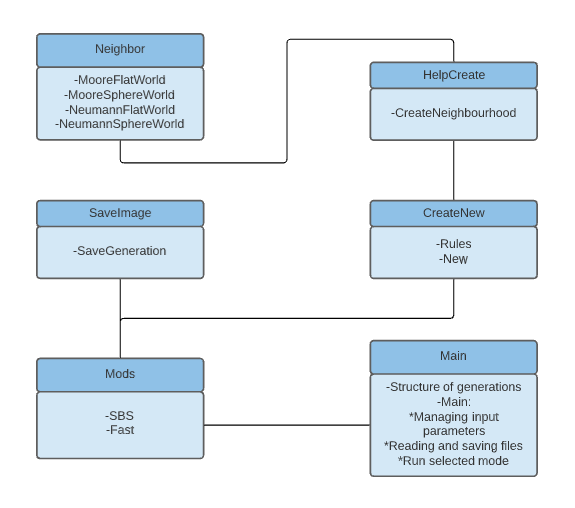
\includegraphics[scale=1.8]{diagram}
\end{figure}

\end{document}
